\documentclass[12pt]{article}

\usepackage[utf8]{inputenc}
\usepackage{newunicodechar}
\newunicodechar{ℝ}{\mathbb{R}}
\usepackage{EngReport}
\usepackage{listings}
\usepackage{cancel}
\usepackage{comment}
\usepackage{amssymb}
\usepackage{amsthm}
\usepackage{amsmath}
\usepackage{graphicx}
\usepackage{setspace}
\usepackage{geometry}
\usepackage{xcolor}  % Required for coloring in listings
\usepackage{tikz}
\usetikzlibrary{automata, positioning, arrows}

\graphicspath{{Images/}}
\onehalfspacing
\geometry{letterpaper, portrait, includeheadfoot=true, hmargin=1in, vmargin=1in}

% Define custom colors
\definecolor{myblue}{RGB}{0, 128, 255}
\definecolor{mygreen}{RGB}{34, 139, 34}
\definecolor{myorange}{RGB}{255, 140, 0}
\definecolor{mygray}{RGB}{128, 128, 128}
\definecolor{mypurple}{RGB}{148, 0, 211}
\definecolor{myred}{RGB}{255, 69, 0}

% Configure listings for Python with custom styles
\lstset{
    language=Python,             % Set language to Python
    basicstyle=\ttfamily\small,  % Use a smaller monospace font
    keywordstyle=\color{myblue}\bfseries,  % Keywords in blue and bold
    commentstyle=\color{mygreen}\itshape,  % Comments in green and italic
    stringstyle=\color{myorange},          % Strings in orange
    numberstyle=\color{mygray},            % Line numbers in gray
    identifierstyle=\color{mypurple},      % Functions and variables in purple
    morekeywords={print, len, range},      % Define additional Python keywords
    showstringspaces=false,                % Do not show spaces in strings
    breaklines=true,                       % Enable line breaking
    numbers=left,                          % Add line numbers to the left
    numbersep=5pt,                         % Space between line numbers and code
    frame=single,                          % Add a box around the code
    rulecolor=\color{mygray},              % Frame color
    moredelim=[is][\color{myred}]{@@}{@@}, % Custom inline LaTeX coloring
}

% Configure the TikZ properties
\tikzset{
    ->,                                         % Make arrows appear directed
    >=stealth,                                  % Make arrow heads bold
    node distance = 3cm,                        % Set min distance between two nodes
    every state/.style={thick, fill=gray!10},   % Configure appearance of nodes in the finite automata
    initial text = $ $                          % Set the text that appears on the start node
}

\begin{document}
\renewcommand{\familydefault}{\rmdefault}

\begin{titlepage}
    \null % This is a TeX command that does nothing but is necessary for vfill to work correctly
    \vfill
    \begin{center}
        {\fontsize{40}{48}\selectfont \bfseries CSC236 Exam Review}
        \vspace{20pt} \\
        {\LARGE Notes from CSC236 Lecture 12} \\
        \vspace{20pt}
        \textbf{Alexander He Meng}
        \vspace{8pt}
        \\ Typed on November 27, 2024
    \end{center}
    \vfill
\end{titlepage}

\pagestyle{fancy}
\fancyhf{}
\setlength{\headheight}{30pt}
\renewcommand{\headrulewidth}{0.4pt}
\renewcommand{\footrulewidth}{0.4pt}
\lhead{\large \textbf{CSC236 UTM} \\ \textbf{Mock Exam }\scriptsize(thx ethan!)\normalsize \textbf{ Solutions}}
\rhead{\large \textbf{Fall 2024} \\ \textbf{Prepared for Dec 17}}
\rfoot{\textbf{Page \thepage}}
\lfoot{}
\pagebreak
\normalsize

\section*{Question \#1}
% Notes:
% - Use the Pumping Lemma to prove non-regularity when needed;
% - Construct DFAs for languages that are regular, focusing on capturing patterns precisely (like binary multiples of 3);
% - Review closure properties (e.g., regular languages are closed under subtraction) to tackle parts involving set differences.
Let $\Sigma = \{ 0, 1 \} $. \\
\\
\textbf{(a):} \\
\textbf{\underline{Claim:}} $\Sigma^*$ is a regular language.
\begin{proof}
\leavevmode\\
    % Provide a DFA that accepts the language in the proof
    % Notes:
    % - It includes every possible string of 0s and 1s;
    % - A DFA can be constructed that accepts any input by having a single accepting state with self-loops for both 0 and 1.
    Let $L_1 = \{0\}$ and $L_2 = \{1\}$ be regular languages of $\Sigma$. \\
    Define $L_3 = L_1 \cup L_2 = \{ 0, 1 \}$ as the regular language obtained by the union of $L_1$ and $L_2$. \\
    \\
    By definition, ${L_3}^*$ is a regular language. Since ${L_3} = \Sigma$, $\Sigma^*$ is also a regular language. \\
    \\
    While this proof is complete, the assignment encourages DFA proofs to show that languages are regular. \\
    \\
    So, as an alternative to \textit{Part (a)}, and for all relevant subsequent parts, adopt a DFA proof. \\
    \\
    Denote the transition function $\delta$ by the following diagram:
    \begin{center}
        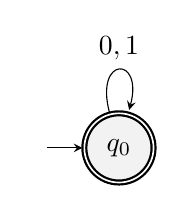
\begin{tikzpicture}[auto]
            \node [state, initial, accepting] (q0) {$q_0$};

            \draw (q0) edge [loop above] node {$0, 1$} (q0);
        \end{tikzpicture}
    \end{center}
    \begin{table}[h!]
        \centering
        \begin{tabular}{|c|c|c|}
            \hline
            \textbf{Old State} & \textbf{Symbol} & \textbf{New State} \\
            \hline
            \( q_0 \) & 0 & \( q_0 \) \\
            \( q_0 \) & 1 & \( q_0 \) \\
            \hline
        \end{tabular}
        \caption{State Transition Table}
    \end{table}
    Using $\delta$, define the deterministic finite automaton $\mathcal{D} = (\mathcal{Q}, \Sigma, \delta, s, F)$, where
    \[
        Q = \{ q_0 \} \text{ is the set of states in } \mathcal{D}
    \]
    \[
        \Sigma = \{ 0, 1 \} \text{ is the alphabet of symbols used by } \mathcal{D} 
    \]
    \[
        \delta : Q \times \Sigma \to Q \text{ is the transition function defined by Table 1}
    \]
    \[
        s = q_0 \text{ is the initial state of } \mathcal{D}
    \]
    \[
        F = \{ q_0 \} \subseteq Q \text{ is the set of accepting states of } \mathcal{D} \text{.}
    \]
    For each state $q_i$, $i \in \{0\}$, in $\mathcal{D}$, define a state invariant $P_q(w)$:
    \[
        P_{q_0}(w): w \text{ is $\epsilon$ or consists of $0$s and $1$s.}
    \]
    As the only state, $q_0$ is trivially mutually exclusive. As well, every string in $\Sigma^* = \{0, 1\}^*$ is either $\epsilon$ or consists of some number of $0$s and $1$s, clearly satisfying $q_0$; exhaustivity is satisfied. \\
    \\
    Let $q \in Q = \{q_0\}$ and $w \in \Sigma^* = \{0, 1\}^*$ both be arbitrary (here, $q = q_0$ always). \\
    Denote the predicate:
    \[
        P_{\delta(q_0, w)}(w) \coloneqq P_q(w) \text{ is the state invariant.}
    \]
    Perform structural induction as follows: \\
    \\
    \underline{Base Case:} \\
    Let $q = q_0$ and $w = \epsilon$. \\
    $P_q(w) = P_{q_0}(\epsilon)$ is true as $w = \epsilon$. \\
    \\
    \underline{Induction Hypothesis:} \\
    Assume that $P_q(w)$ is true for all $q \in \{q_0\}$ and some $w \in \{0, 1\}^*$. \\
    This means $w$ is either empty or consists of $0$s and $1$s. \\
    \\
    \underline{Induction Step}: \\
    Demonstrate that all state invariants hold when processing strings from the $\Sigma = \{0, 1\}$. \\
    This can be achieved by showing that $P_{\delta(q, z)}(wz)$ holds for all $q \in \{q_0\}$ and $z \in \{0, 1\}$. \\
    \\
    Let $w \in \{0, 1\}^*$ be arbitrary. \\
    \\
    Let $q = q_0$, $z \in \{0, 1\}$, and assume $P_{q_0}(w)$ is true. \\
    Notice that $\delta(q, z) = \delta(q_0, 0) = q_0$. Conveniently, $P_{q_0}$ is already true by assumption. \\
    \\
    There are no other state invariants in $\mathcal{D}$. By the principle of structural induction, $P_{\delta(q_0, w)}$ is true for all $q \in Q = \{q_0\}$ and $w \in \Sigma^* = \{0, 1\}^*$. \\
    \\
    Finally, demonstrate that $\mathcal{D}$ accepts exactly the language $L = \Sigma^*$ over $\Sigma = \{0, 1\}$. \\
    This is achievable by showing that if $w \in \Sigma^* = \{0, 1\}^*$ is arbitrary, $w$ is a member of $L$ if and only if there exists an accepting state $q \in F$ such that $P_q(w)$ holds. \\
    \\
    By the definition of $P_{q_0}(w): \text{$w$ is $\epsilon$ or consists of $0$s and $1$s}$. \\
    If $w \in L$, then it is either an empty string or consists of $0$s and $1$s. Clearly, $P_{q_0}(w)$ must be true. \\
    On the other hand, choose the accepting state $q_0 \in F$ and assume $P_{q_0}(w)$ is true. Clearly, $w \in L$, due to matching definitions. \\
    \\
    Therefore, while this DFA proof is redundant in nature, it is clear that $\mathcal{D}$ accepts $L = \Sigma^*$ over $\Sigma = \{0, 1\}$. \\
    Again, $L = \Sigma^*$ is demonstrated to be a regular language. \\
\end{proof}
\leavevmode\\
\textbf{(b):} \\
\textbf{\underline{Claim:}} $\Sigma^* \setminus K, K = \{ 01, 101, 010 \}$ is a regular language.
\begin{proof}
\leavevmode\\
    % Provide a DFA that accepts the language in the proof
    % Notes:
    % - Regular languages are closed under finite set differences;
    % - K is finite, so the difference \Sigma^*\setminus{K} is also regular;
    % - A DFA can be constructed that accepts all strings except specific patterns 01, 101, and 010.
    This proof aims to show that the language $\Sigma^* \setminus K$ is a regular language by constructing a DFA that accepts all strings except the literal strings in $K = \{ 01, 101, 010 \}$. \\
    \\
    Denote the transition function $\delta$ by the following table:
    \begin{table}[!h]
        \centering
        \begin{tabular}{|c|c|c|}
            \hline
            \textbf{Old State} & \textbf{Symbol} & \textbf{New State} \\
            \hline
            % had empty string (check prefix)
            \( q_\epsilon \) & 0 & \( q_0 \) \\
            \( q_\epsilon \) & 1 & \( q_1 \) \\
            \hline
            % had 0
            \( q_0 \) & 0 & \( q_5 \) \\
            \( q_0 \) & 1 & \( q_2 \) \\
            \hline
            % had 1
            \( q_1 \) & 0 & \( q_4 \) \\
            \( q_1 \) & 1 & \( q_5 \) \\
            \hline
            % had 01
            \( q_2 \) & 0 & \( q_3 \) \\
            \( q_2 \) & 1 & \( q_5 \) \\
            \hline
            % had 010 or 101 (accepts on next)
            \( q_3 \) & 0 & \( q_5 \) \\
            \( q_3 \) & 1 & \( q_5 \) \\
            \hline
            % had 10
            \( q_4 \) & 0 & \( q_5 \) \\
            \( q_4 \) & 1 & \( q_3\) \\
            \hline
            % guaranteed accepting
            \( q_5 \) & 0 & \( q_5 \) \\
            \( q_5 \) & 1 & \( q_5 \) \\
            \hline
        \end{tabular}
        \caption{State Transition Table}
    \end{table}
    Using $\delta$, define the DFA $\mathcal{D} = (\mathcal{Q}, \Sigma, \delta, s, F)$, where
    \[
        \mathcal{Q} = \{ q_0 \} \text{ is the set of states in } \mathcal{D}
    \]
    \[
        \Sigma = \{ 0, 1 \} \text{ is the alphabet of symbols used by } \mathcal{D}
    \]
    \[
        \delta : \mathcal{Q} \times \Sigma \to \mathcal{Q} \text{ is the transition function define by Table 2}
    \]
    \[
        s = q_0 \text{ is the initial state of } \mathcal{D} 
    \]
    \[
        F = \{ q_2, q_3 \} \subseteq \mathcal{Q} \text{ is the set of accepting states of } \mathcal{D} \text{.}
    \]
    For each state in $\mathcal{D}$, define a state invariant $P_q(w)$, describing the property of any string $w \in \Sigma^*$ which leads $\mathcal{D}$ to state $q$:
    \[
        P_{q_\epsilon}(w): 
    \]
    \[
        P_{q_0}(w): 
    \]
    \[
        P_{q_1}(w): 
    \]
    \[
        P_{q_2}(w): 
    \]
    \[
        P_{q_3}(w): 
    \]
    \[
        P_{q_4}(w): 
    \]
    \[
        P_{q_5}(w): 
    \]
\end{proof}
\leavevmode\\
\textbf{(c):} \\
\textbf{\underline{Claim:}} $\{ w | w \text{ is a palindrome} \}$ is NOT a regular language.
\begin{proof}
\leavevmode\\
    % Notes:
    % - Palindromes require matching symbols from opposite ends of the string, which requires memory beyond finite states;
    % - The Pumping Lemma can be used here to show non-regularity (if that is taught).
    proofgoeshere \\
\end{proof}
\leavevmode\\
\textbf{(d):} \\
\textbf{\underline{Claim:}} $\{ ww | w \in \Sigma* \}$ is NOT a regular language.
\begin{proof}
\leavevmode\\
    % Notes:
    % - Recognizing it would require counting to ensure that both halves are the same, but that is beyond a finite automaton's capability;
    % - The Pumping Lemma can also prove this non-regularity.
    proofgoeshere \\
\end{proof}
\leavevmode\\
\textbf{(e):} \\
\textbf{\underline{Claim:}} $\{ w | ww \in \Sigma* \}$ is a regular language.
\begin{proof}
\leavevmode\\
    % Notes:
    % - Any string w such that its concatenation with itself (i.e. ww) is in \Sigma* means w can be any string over {0, 1};
    % - This set includes all strings in \Sigma*, so it's equivalent to \Sigma*, which is regular.
    proofgoeshere \\
\end{proof}
\leavevmode\\
\textbf{(f):} \\
\textbf{\underline{Claim:}} $\{ w | w \text{ is a binary representation of a multiple of 3} \}$ is a regular language.
\begin{proof}
\leavevmode\\
    % Notes:
    % - A DFA can be constructed to recognize binary representations of multiples of 3, as shown in formal language theory;
    % - This DFA works by keeping track of remainders modulo 3, which requires only a finite number of states (three states, one for each possible remainder).
    proofgoeshere \\
\end{proof}
\leavevmode\\
\pagebreak

\section*{Question \#2}
\textbf{\underline{Claim:}} Regular expressions that also have access to complement can still only express the same class of languages (i.e. the class of regular langauges) as regular expressions without the complement operation.
\begin{proof}
\leavevmode\\
    % Notes:
    % - Argue that a regular language's closure properties (under union, intersection, and complement) enable the construction of an equivalent regular expression without changing the language class.
    % - Construct examples to illustrate equivalency using De Morgan's laws and closure proofs.
    Suppose $r$ is an arbitrary regular expression with alphabet $\Sigma$ so that $L = \mathcal{L}(r)$ is a regular language. \\
    Assume $r$ has access to the complement operation. \\
    \\
    Let $\overline{L} = \{ x \in \Sigma^* \mid x \notin L \}$ be the regular language representing the \textit{complement} of L. \\
    Assume $\overline{r}$ is a regular expression, with $\mathcal{L}(\overline{r}) = \overline{\mathcal{L}(r)}$. \\
    \\
    By definition, there exists a DFA $\mathcal{M}$ that accepts $L$. \\
    \\
    Construct $\mathcal{M}$: \\
    \(\mathcal{M} = (Q, \Sigma, \delta, s, F)\), where
    \begin{itemize}
        \item Q is a set of finite states;
        \item $\Sigma$ is the alphabet;
        \item $\delta : Q \times \Sigma \to Q$ is the transition function;
        \item $s$ is the start state;
        \item $F \subseteq Q$ is the set of accepting states.
    \end{itemize}
    \leavevmode\\
    Next, define $\overline{L} = \Sigma^* \setminus L$ as the regular language containing everything obtainable from the alphabet $\Sigma$ except members of $L$. \\
    \\
    Construct $\overline{M}$ to be identical to $M$, except for its accepting states:
    \begin{itemize}
        \item Q is a set of finite states;
        \item $\Sigma$ is the alphabet;
        \item $\delta : Q \times \Sigma \to Q$ is the transition function;
        \item $s$ is the start state;
        \item $Q \setminus F \subseteq Q$ is the set of accepting states.
    \end{itemize}
    \leavevmode\\
    Notice that $\overline{M}$ share the same states, alphabet, transition function, and start state as those of $M$. The difference is the set of accepting states in $\overline{M}$, which is designed to be mutually exclusive from that of $M$. \\
    \\
    \textbf{Self-Note: now add the proof that $\overline{M}$ accepts $\overline{L}$, and connect it back to regexes.}
    \\
    Next, let $\overline{r}$ be some regular expression without the complement operation.

\end{proof}
\pagebreak

\section*{Question \#3}
\textbf{Counter-free languages} are a subset of languages that satisfy the condition:
\[
    (\exists n \in \mathbb{N})(\forall x, y, z \in \Sigma^*)(\forall m \geq n)(xy^mz \in L \iff xy^nz \in L) \text{.}
\]
\textbf{Star-free regular expressions} are regular expressions without the Kleene star, but with complementation. \\
\\
It is known in formal language theory that counter-free languages are equivalent to the languages that can be expressed as \textbf{star-free regular expressions}. \\
\\
\textbf{(a):} \\
\textbf{\underline{Claim:}} $(ab)^*$ can be matched with a star-free regular expression, where $\Sigma = \{ a, b \}$.
\begin{proof}
\leavevmode\\
    % Notes:
    % - Find a star-free regular expression for (ab)*.
    The expression $(ab)^*$ represents strings in the set $\{ \epsilon, ab, abab, ababab, \dots\}$. \\
    \\
    This means matching strings are strings where every occurrence of $a$ is immediately followed by a $b$. \\
    \\
    Due to the definition of $\Sigma = \{ a, b \} $, an equivalent star-free regular expression can be written in terms of the complement. The complement definition is highlighted below:
    \begin{itemize}
        \item The string starts with $b$ if it is not empty;
        \item The string contains an $a$ not immediately followed by a $b$.
    \end{itemize}
    As a regular expression, this is $?$. \\

\end{proof}
\leavevmode\\
\textbf{(b):} \\
\textbf{\underline{Claim:}} $(ab)^*$ is a counter-free language, where $\Sigma = \{ a, b \} $. 
\begin{proof}
\leavevmode\\
    % Notes:
    % - Use the definition of counter-free langauges to show that (ab)* satisfies the condition for counter-freeness.
    By definition, if $(ab)^*$ is a counter-free language, there exists natural $n$ for all $x, y, z \in \{ a, b \}^*$ and for all $m \geq n$ such that $xy^mz \in (ab)^* \iff xy^nz \in (ab)^*$. \\
    \\
    Let $n \in \mathbb{N}$. Let $x, y, z \in \{ a, b \}^*$ and $m \geq n$ both be arbitrary. \\
    \\
    \underline{Show that $xy^mz \in (ab)^* \implies xy^nz \in (ab)^*$:} \\
    Suppose $xy^mz \in (ab)^*$. \\
    \\
    Since $m \geq n$ is arbitrary,  \\
    \\
    a \\
    \\
    \underline{Show that $xy^mz \in (ab)^* \impliedby xy^nz \in (ab)^*$:} \\
    \\
\end{proof}
\leavevmode\\
\textbf{(c):} \\
\textbf{\underline{Claim:}} $(aa)^*$ is NOT a counter-free language, where $\Sigma = \{ a \} $. 
\begin{proof}
\leavevmode\\
    % Notes:
    % - Find a counterexample to the condition, demonstrating the need for counting.
    proofgoeshere \\
\end{proof}
\pagebreak

\section*{Question \#4}
Let $k \in \mathbb{N}$ be arbitrary. Let $w \in \Sigma^*$, where $|\Sigma| \geq 2$ and has $1$ as one of its symbols. \\
\\
Consider the language $L = \{ w | \text{the $k^\text{th}$ to last character of $w$ is $1$} \}$. \\
\\
% Notes (raw):
% For part (a), apply state counting arguments using the DFA properties for strings of length kk.
% Part (b) involves constructing a minimal NFA and proving it has kk states, focusing on non-deterministic behavior that simplifies the automaton.
% The bonus in part (c) requires DFA minimization techniques; try to show the necessity of 2k+1−12k+1−1 states by reasoning about state distinguishability.
\textbf{(a):} \\
\textbf{\underline{Claim:}} A DFA that accepts $L$ has to have at least $2^k$ number of states.
\begin{proof}
\leavevmode\\
    \textbf{ACTUALLY, SHOW THIS BY CONTRADICTION: Suppose whatever... less than $2^k$ states.} \\
    \\
    A DFA is determinstic and requires states to remember the ``history'' of the input. For the language $L = \{ w | \text{the $k^\text{th}$ to last character of $w$ is $1$} \}$, the DFA must track the last $k$ characters of the input string. \\
    \\
    Notice that there are $2^k$ possible combinations of $k$-length binary substrings, and each of these combinations must map to a unique state in the DFA for accurate processing. \\
    \\
    Any DFA with fewer than $2^k$ states cannot differentiate between all possible $k$-length suffixes, causing the automaton to classify strings incorrectly. \\
    \\
    Any DFA with more than $2^k$ states either accepts $L$ with a larger alphabet with more than $2$ symbols, or is introducing repetitive and redundant states, but still works. \\
\end{proof}

\leavevmode\\
\textbf{(b):} \\
\textbf{\underline{Claim:}} The smallest NFA that accepts $L$ has to have exactly $k$ number of states.
\begin{proof}
\leavevmode\\
    In an NFA, non-determinism allows the automaton to ``guess'' when it is $k$-steps away from the end of the string. \\
    \\
    The NFA for $L$ needs only $k$ states because:
    - The start state (initial state) represents the starting position;
    - The NFA transitions through $k - 1$ intermediate states to track progress. \\
\end{proof}
\leavevmode\\
\textbf{(c):} \\
\textbf{\underline{Claim:}} The smallest DFA that accepts $L$ has to have exactly $2^{k + 1} - 1$ number of states.
\begin{proof}
\leavevmode\\
    proofgoeshere \\
\end{proof}
\leavevmode\\
\pagebreak

\section*{Question \#5}
\textbf{\underline{Claim:}} Every finite language can be represented by a regular expression (meaning all finite languages are regular).
\begin{proof}
\leavevmode\\
    Let $\Sigma$ be an arbitrary alphabet. Let $L$ be an arbitrary finite language over $\Sigma$. \\
    \\
    Let $n$ be an arbitrary natural number. \\
    Denote the predicate:
    \[
        P(n) \coloneqq |L_n| = n \implies \text{$L_n$ can be represented as a regular expression.}
    \]
    \\
    This proof uses the principle of simple induction to show $P(n)$ for all $n \in \mathbb{N}$. \\
    \\
    \underline{Base Cases:} \\
    Let $n = 0$. \\
    This means $|L_n| = 0$, so $L_n = \emptyset$. By definition, the empty set is a regular expression. \\
    Thus, $P(0)$. \\
    \\
    Let $n = 1$. \\
    Then $|L_n| = 1$, so $L_n = \{ w \}$ for some string $w \in \Sigma^*$. By definition, any single string over an alphabet is a regular expression. \\
    Thus, $P(1)$. \\
    \\
    \underline{Induction Hypothesis} \\
    Assume that $P(k)$ holds for some natural $k$. \\
    \\
    This means if $L_k$ has $k$ strings, then $L_k$ can be represented as a regular expression. \\
    \\
    \underline{Induction Step:} \\
    Let $L_{k + 1} = \{ w_1, w_2, \dots, w_k, w_{k + 1} \}$, where $w_i \in \Sigma^*$ for $i \in [1, k + 1] \cap \mathbb{N}$. \\
    \\
    By the Induction Hypothesis, $L_k = L_{k + 1} \setminus \{ w_{k + 1} \} = \{ w_1, w_2, \dots, w_k, w_{k + 1} \} \setminus \{ w_{k + 1} \} = \{ w_1, w_2, \dots, w_k \}$ has language has regular expression $r_k$ such that $L_k = \mathcal{L}(r_k)$. \\
    \\
    Notice that:
    \begin{itemize}
        \item The regex $r_k$ represents the language $L_k$;
        \item The regex $w_{k + 1}$ represents the language $\{ w_{k + 1} \}$.
    \end{itemize}
    Then, $L_{k + 1}$ can be constructed as a regex as follows:
    \[
        L_{k + 1} = L_k \cup \{ w_{k + 1} \}
    \]
    By definition, the union of two regexes is a regex. Construct $r_{k + 1}$:
    \[
        r_{k + 1} = r_k + w_{k + 1}
    \]
    As desired, the regex $r_{k + 1}$ represents the language $L_{k + 1}$. \\
    \\
    \underline{Conclusion:} \\
    By the principle of simple induction, $P(n)$ holds for all $n \in \mathbb{N}$. It follows that all finite languages must be regular. \\
\end{proof}
\pagebreak

\end{document}
